\hypertarget{group__dns}{}\section{D\+NS}
\label{group__dns}\index{D\+NS@{D\+NS}}
Collaboration diagram for D\+NS\+:
\nopagebreak
\begin{figure}[H]
\begin{center}
\leavevmode
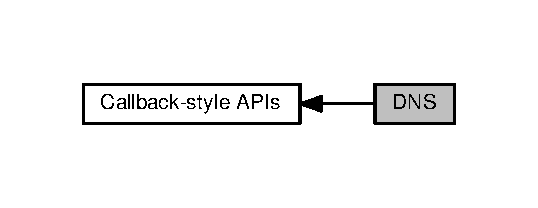
\includegraphics[width=258pt]{group__dns}
\end{center}
\end{figure}
Implements a D\+NS host name to IP address resolver.

The lw\+IP D\+NS resolver functions are used to lookup a host name and map it to a numerical IP address. It maintains a list of resolved hostnames that can be queried with the dns\+\_\+lookup() function. New hostnames can be resolved using the dns\+\_\+query() function.

The lw\+IP version of the resolver also adds a non-\/blocking version of gethostbyname() that will work with a raw A\+PI application. This function checks for an IP address string first and converts it if it is valid. gethostbyname() then does a dns\+\_\+lookup() to see if the name is already in the table. If so, the IP is returned. If not, a query is issued and the function returns with a E\+R\+R\+\_\+\+I\+N\+P\+R\+O\+G\+R\+E\+SS status. The app using the dns client must then go into a waiting state.

Once a hostname has been resolved (or found to be non-\/existent), the resolver code calls a specified callback function (which must be implemented by the module that uses the resolver).

Multicast D\+NS queries are supported for names ending on \char`\"{}.\+local\char`\"{}. However, only \char`\"{}\+One-\/\+Shot Multicast D\+N\+S Queries\char`\"{} are supported (R\+FC 6762 chapter 5.\+1), this is not a fully compliant implementation of continuous m\+D\+NS querying!

All functions must be called from T\+C\+P\+IP thread.

\begin{DoxySeeAlso}{See also}
\hyperlink{group__netconn__common}{Common functions} for thread-\/safe access. 
\end{DoxySeeAlso}
